\documentclass[]{llncs}   % list options between brackets

\usepackage{color}
\usepackage{graphicx}
\usepackage{subcaption}
\usepackage{amssymb}
\usepackage{standalone}
\usepackage{pgfplots}
\usepackage{amsmath}
\usepackage{tikz}

\usepackage{listings}

\usepackage{hyperref}

\usepackage{systeme}

\usepackage{enumitem}

\usepackage{float}

\def\shownotes{1}
\def\notesinmargins{0}

\ifnum\shownotes=1
\ifnum\notesinmargins=1
\newcommand{\authnote}[2]{\marginpar{\parbox{\marginparwidth}{\tiny %
  \textsf{#1 {\textcolor{blue}{notes: #2}}}}}%
  \textcolor{blue}{\textbf{\dag}}}
\else
\newcommand{\authnote}[2]{
  \textsf{#1\textcolor{blue}{ #2}}}
\fi
\else
\newcommand{\authnote}[2]{}
\fi

\newcommand{\knote}[1]{{\authnote{\textcolor{green}{Alex notes:}}{#1}}}
% type user-defined commands here

\usepackage[T1]{fontenc}
\usepackage{xcolor}

\definecolor{dkgreen}{rgb}{0,0.6,0}
\definecolor{gray}{rgb}{0.5,0.5,0.5}
\definecolor{mauve}{rgb}{0.58,0,0.82}

\pgfplotsset{compat=newest, table/search path=figures}

\begin{document}

\title{On Contractual Money}

\author{Alexander Chepurnoy\inst{1,2}, Amitabh Saxena\inst{1}}
\institute{Ergo Platform \\\email{\{kushti\}@protonmail.ch}}

\maketitle

\section{Abstract}

It is common to consider such functions of money as medium of exchange, store of value, unit of account.
In this work we highlight another function of money. That is, money can act as units of contract execution. 
Historically, there is always some implicit or strictly defined paper contract behind the money.
However, with the rise of cryptocurrencies, we now have `programmable money', where it is easy to bind digital assets to an explicit contract. We use the term {\em contractual money} to refer to digital money with a usage contract provided in the form of executable code. In the first and still the most popular cryptocurrency, Bitcoin, a coin is bound to a contract which combines
statements about secret data~(such as {\em provide a signature on spending transaction bytes that verifies under the public key $pk$}) and predicates on blockchain data at the time of contract execution (i.e., transaction validation).  Bitcoin allows predicates only on two variables from blockchain data, namely timestamp and blockchain height, which makes its contracts very restrictive.
However, with certain context extensions, including the spending transaction itself, it becomes possible to execute
arbitrarily complex programs, allowing us to implement contractual money on top of a Bitcoin-like cryptocurrency. We demonstrate this via examples.
In the first example, a private scrip is issued for a microcredit use-case. A contract enforces that the borrower spend a certain amount of the scrip money only as described in the contract. For instance, the borrower has to spend at least 50\% of the money on equipment by buying it from a white-listed party and 20\% on construction works, again, using a predefined white-list. For privacy, the identities of selected white-listed parties are protected via ring signatures. We provide code for such contract implemented on top of Ergo cryptocurrency. In the second example, money is issued by a local government with the aim of providing local job guarantees and promoting development of local economy. To achieve this, the government pays for communal works at the rate of one token per hour, with each token backed by a fixed amount of national currency. The tokens can be spent in arbitrary ways, but can only be exchanged for national currency by a local producer from a white-list. This is simple enough to work with paper based contracts but digital implementations allow enhanced contracts with additional possibilities. We also review the famous Woergl experiment, where, according to data published by Von Muralt in 1934, the main reason for success was not the demurrage component of the Woergl money. Rather, the experiment was a scheme to convert local tax debts into communal works, with demurrage speeding up~(and, to some degree, enforcing) the process. We conclude by describing a {\em Local Exchange Trading System} (LETS) contract implemented on top of the Ergo blockchain. To the best of our knowledge, this is the first implementation of LETS using a blockchain.


\section{Introduction}
\label{sec-intro}
 
Bitcoin~\cite{Nakamoto2008} was introduced in 2008 by Satoshi Nakamoto as a peer-to-peer currency which ledger is
written into blockchain, a database which is fully replicated across the network peers and making progress without a trusted
party or expensive coordination while majority of peers solving proof-of-work puzzles are honest.

Originally, digital coins~(of arbitrary nominal) in the Bitcoin ledger were associated with public keys. That is, in order
to spend a coin, owner of a private key corresponding to the public key of the coin should provide a signature for a
spending transaction, and validity of the signature could be checked by Bitcoin peers by using the public key~(and the spending transaction).
Soon after the launch, Bitcoin adopted somewhat programmability, thus a coin is bound to a contract, which combines
statements about secret data~(such as ``valid proof of private key knowledge associated with the public key $pk$
against spending transaction bytes is needed to be provided'') with predicates on blockchain
data~(to be validated in peer-to-peer network without trusted authority, transaction validation could not involve
data external to the blockchain, as the only data peers are agreed on when verifying a block with the transaction
is the blockchain before this block and the block itself).

A popular trend of cryptocurrencies which was started with Bitcoin launched in 2009 brought two new exciting features.
In the first place, a cryptocurrency is decentralized, which mean that, at least, its minting process is permissionless.
In the second place, cryptocurrencies allow to programmability to some extent; unlike a coin or a note in the physical
world, or digital representation of fiat money in bank accounts, a digital coin~(of arbitrary denomination) in Bitcoin
is protected by a guarding script.

It is common to consider such functions of money as medium of exchange, store of value, unit of account, and so on.
In this work we highlight another function of money. That is, money can act as units of contract execution.

This function is implicitly exists since the very early days of money history. A very clear historical example of paper money associated with a contract is Hundis~\cite{martin2009hundi}. A modern example could be found in
maternity capital in Russia: the government is giving a certificate associated with some amount of national fiat currency~(rubles)
to mothers of two and more children. Unlike fiat currency, the maternity capital money could be spent on particular
topics only, like children's education or housing improvement.

However, with cryptocurrencies it becomes easy to make a digital coin~(of arbitrary nominal) which use cases are
explicitly bounded by a contract in form of executable code stored in the coin itself.

Bitcoin first made that move with a simple
scripting language named Bitcoin Script which allows some programmability: a coin could be spent if its protecting script,
given arguments provided by spending transaction, and also height and timestamp of the block which contains the
transaction~\footnote{Height and timestamp were added in Bitcoin 0.11},
is being evaluated to $true$ value. A newer cryptocurrency Ergo~\cite{ergowp} is going further with spending transaction~(along with other additional
fields) fully projected into the execution context. This enhancement allows to execute even any Turing-complete
contract~\cite{chepurnoy2018self}. In financial applications, it allows to create a coin which could be spent only by
a transaction which creates a coin with specific properties. In the same fashion, a coin may require a chain of
transactions, or a coin may create a family of coins with specific properties. Thus it is possible to create money~(in
form of contractually bound Ergs or auxiliary tokens as it is possible to explicitly create a token in Ergo) bounded by a contract 
, which possibly has many states. 

The main distinguishing point of contractual money is embedding of its contract, which existed externally (in form of laws, corporate terms, informal and often implicit person-to-person agreements), directly into the unit of money. Thus money being created with a specific contract are enforcing its users to follow the contract precisely. Other functions of money (medium-of-exchange, store-of-value, unit-of-account) could be precisely shaped by the contract and thus become secondary.

The paper is organized as follows. Section~\ref{sec-txmodel} describes transactional model of Bitcoin and Ergo. Then the paper provides few motivating examples for contractual money. Section~\ref{sec-microcredit} provides an example of one-time microcredit money. Section~\ref{sec-combination} sketches a currency which combines properties of time and local currencies. Section~\ref{sec-worgl} reflecting the famous W\"{o}rgl experiment from contractual money point of view. Section~\ref{sec-lets} describes two possible Local Exchange Trading System implementations on top of a blockchain, one with a trusted committee while another is using no trusted committee but cryptocurrency collaterals in order to secure debts. With Section~\ref{sec-conslusion} we conclude.


\section{Key Contractual Aspects of Bitcoin and Ergo}
\label{sec-txmodel}

In Bitcoin, a `coin' contains some quantity of tokens known as {\em satoshis}. All coins are stored in short-lived immutable objects called {\em Unspent Transaction Outputs} (UTXOs). 
A UTXO contains an {\em amount} representing the quantity of tokens locked in it and an {\em locking script} representing the requirements under which the tokens may be spent (for instance, it can require a signature on the transaction). Thus, a UTXO can be thought of as a locked box with some tokens inside and the act of spending the UTXO can be thought of as unlocking the box.
The actual state of Bitcoin then is the entire UTXO set. 

A transaction modifies this state by spending existing UTXOs as {\em inputs} and creating new ones as {\em outputs}. 
Bitcoin transactions adhere to a weak conservation law: the total number of tokens in the outputs may be less than or equal to that in the inputs (the exception is a reward transaction that generates new tokens).

Each input UTXO must be accompanied by an {\em unlocking script} that convinces everyone that the condition specified by the locking script is satisfied. For instance, this can be a signature on the transaction. Both scripts executed together determine determine the transaction's validity.
Figure~\ref{fig1} shows how a Bitcoin transaction works.
\begin{figure}
	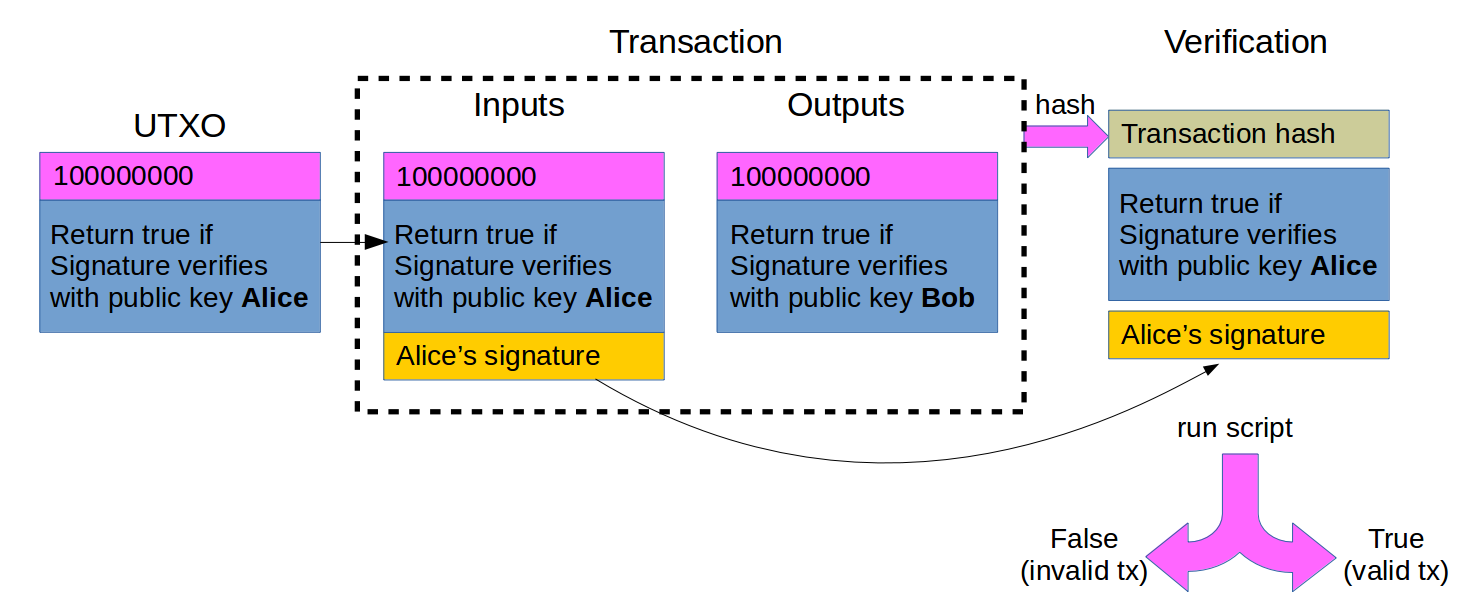
\includegraphics[scale=0.24]{bitcoin}
	\caption{Verifying a Bitcoin transaction}
	\label{fig1}
\end{figure}

Bitcoin's locking script can require signatures from multiple parties and also refer to context variables (the state of the blockchain). Currently, the only context variables allowed in Bitcoin are the height and time. 

Ergo is also based on the same model and a UTXO is called a {\em box} in Ergo. In addition to the amount and locking script, a box can also store additional data in {\em registers}. Ergo context has the entire spending transaction and the block solution. Thus, an Ergo contract can refer to other inputs and outputs of the transaction. For instance, we can require that certain inputs or outputs must have some structure, such as being protected by a given script. This allows creating even Turing-complete contracts~\cite{chepurnoy2018self}. In addition to the primary token, a box can contain some secondary tokens.
Each transaction can create arbitrary quantity of exactly one secondary token, whose id is given by the box id of the first input. Ergo follows the strong conservation rule (exactly equal) for the primary token and the weak rule (less than or equal) for secondary tokens. 

\section{One-Time Microcredit Money}
\label{sec-microcredit}

 In this section we consider a private digital scrip issued in order to serve needs of a specific credit contract. Thus money behind the credit contract are enforced to be spent as prescribed by precise rules of the contract.

 For example, we assume that a lender in India is providing a small loan to an entrepreneur to help him in establishing a business.
 A common source of risk in this field is lying during loan application, and also reckless spending of credit funds~(for example, on prestigious consumer goods instead of business tools). To reduce risks, microcredit
 organizations are even holding financial literacy trainings for clients~\cite{finliteracy}. This problem could be tackled with by  enforcing a borrower to spend money exactly on needs declared in the application form.  

 Assume that a borrower is claiming in the application form that he will spend half of a loan of $100,000$~(or one lakh) 
 Indian Rupees in total on equipment, $20,000$ will be spent on constructing a building where production will happen, while the rest will be spent in arbitrary way or sit in reserves to tackle unexpected problems.

 Thus the lender is creating a digital token backed in 1:1 way by Indian Rupees, we name it IMTIR~(Individual Microcredit Token backed by Indian Rupee). Assume that there are four equipment sellers known to the lender in the area, named $E1$, $E2$, $E3$, $E4$, and
 there are three builders also, $B1$, $B2$, $B3$. All the $100,000$ tokens could be stored in one coin initially, and the coin usage is bounded by the following contract:

 \begin{enumerate}
    \item{} The lender is creating $100,000$ IMTIRs in form of a digital coin.
    \item{} When spending a coin, the borrower has to spend at least $50,000$ IMTIRs to one of $E1$, $E2$, $E3$, $E4$, and
    at least $20000$ IMTIRs to one of $B1$, $B2$, $B3$. After this initial spending, IMTIRS could be spent in arbitrary way.
\end{enumerate}

 After this simple contract being done, IMTIRs could be exchanged with Rupees, for example, via a digital asset exchange. The borrower
 pay the loan back in Rupees as usually. 

 This basic contract could be enhanced in many ways. For example, the loan could be made in interest-free way. That is,
 the lender may exchange money with a discount, or introduce a demurrage~(or combine both). For example, the borrower may pay 
 0.97 Rupees per 1 IMTIR. Still, the businesses would probably like to participate in this scheme to get an increased money flow coming through~(even with less profit). Thus the lender may get profit from businesses soon, and then it is enough to get loan paid out with no interest by the borrower. However, this could be the case only if currency of the loan has no inflation. This is not the case for most of fiat currencies. What the lender and the borrower can do in this case is to use a trusted provider of statistical
 information, namely, inflation indicators. Then the lender and the borrower may fix loan in prices on approval date.

  Then a contract~\footnote{Please note that we omit a demurrage component from
 the contract.} behind IMTIR money, with the underlying interest-free loan approved on Jan, 1st, 2020,
 could be as follows: ``the borrower is paying out the debt without the interest by buying IMTIR tokens with digitalized Indian Rupees, using inflation data from trusted oracle''.
 
 In the example IMTIR is acting as contractual money currency bounded by the loan contract, with intentionally limited by a
 program medium-of-exchange functionality. A contract code which is similar to basic IMTIR case is described in~\cite{scpeople}.

 However, IMTIR token flows are not private on the blockchain. In order to protect privacy of the lender, the borrower
 may issue every month tokens which are backed by Indian Rupees~(in prices for the beginning of the month). In our example, the
 borrower can provide a loan in MTIR-01-2020~(Microcredit Tokens backed by Indian Rupee in prices of
 Jan, 2020) tokens. To protect privacy of the spending (to one of $B1$, $B2$, $B3$, and one of $E1$, $E2$, $E3$, $E4$), ring
 signatures~\cite{rivest2001leak} can be used.

 MTIR-01-2020 tokens could also be made freely tradeable~(on exchanges). That is, the lender must repay the loan in
 digitalized Rupees, and the borrower is always selling enough MTIR-01-2020 tokens for Rupees, with exchange rate equals
 to, for example, official inflation since issuance of the tokens. However, if another agent is experiencing lower inflation
 than the borrower, he can buy at the lower price and then make profits from arbitrage.

\section{Combination of time and local currencies}
\label{sec-combination}

Local and regional currencies, such as Chiemgauer~\cite{thiel2011complementary} and Berkshares~\cite{swann1995local}, are developed to increase money velocity within the local economy.

A complementary currency for local job guarantee has been proposed by Forstarter in~\cite{forstater2018complementary} as a mean
of job creation by using the complementary currency to pay for community service employment.

In this example, we show how to create a contractual currency which is intended to solve both problems of low
employment and stagnation of local economy. We will refer to the currency as to LCJC (local community job currency).

For example, a local government in Russia may issue certificates, where each certificate is equals to 1 hour of community work, and also 200 Rubles. Each certificate is a digital coin, which could be converted into Rubles only by white-listed local manufactures, so a worker may spend them in any way but LCJC Rubles could be transformed into Rubles only by approved manufacturers.

In rural areas, the system could be run even without a digital contracts. However, in a digital form there could be
additional properties achieved, for example,
    \begin{itemize}
        \item{} a demurrage component may be added to increase money velocity. However, demurrage can be implemented over paper 
        certificates as well, as it was done in the W\"{o}rgl experiment, but when a coin exists in digital form 
         demurrage fee can be charged with no need to visit an office every month.
        \item{} as digital money could be traceable on the way from employers to local producers, an additional
        requirements could be made against the money flow. For example, it could be required for money to get through
        white-listed shops (from a designated list) to get to a producer. Also, it could be required for a shop, and also for a
        producer to send 1 percent of LCJC volume (each) to local charity organizations.
    \end{itemize}


With LCJC currency as a warm-up, we are ready to revisit the famous W\"{o}rgl experiment.

\section{The W\"{o}rgl Experiment}
\label{sec-worgl}

The W\"{o}rgl experiment covered in~\cite{muralt1934woergl} is well-known successful example of a local currency. In
contrary to most of the writings suggest that the currency was able to revive the local economy because of demurrage, we
 note that the experiment was a successful scheme to convert local tax debts into building community projects, with
 local businesses being fueled with money on the way. Moderate success of current regional currencies with demurrage~\cite{thiel2011complementary} is a particular sign that demurrage itself is not a silver bullet for solving problems of local economies.
 With that in mind, original paper of Von Muralt~\cite{muralt1934woergl} is to be revisited. 

 The first question to be answered is how ``relief money''~(a term by Von Muralt) were issued. The answer from the original paper is clear: ``the depreciating money was brought into circulation by the parish paying its clerical and manual workers, at first 50\% and later 75\% of their remuneration, in relief money''. As only local businesses accepted the relief money, the scheme looks like LCJC 
 currency from the previous section. 

 However, issuance of the money did not create inflation, per Von Muralt, ``no rise in prices appears to have occurred''. The reason behind that, according to data in the paper, is that most of the money quickly returned back to parish in order to pay local tax debts. According to the paper, ``the important indirect gain of the system lies, according to the burgomaster, in that already during the first six months heavy tax arrears, 90\% of these in relief money, reached the parish treasury.''. Because of that, it became unnecessary to increase initial collateral~(in form of bank deposit) backing issued relief money. Demurrage helped businesses to pay taxes as soon as possible~(sometimes, in advance). 

 Thus W\"{o}rgl experiment could be represented as a scheme of converting tax debts into communal work~(such as repaired roads of the town). A contract for the experiment could be trivially stated explicitly and digitalized.

\section{Local Exchange Trading System}
\label{sec-lets}

A local exchange trading system (LETS)\cite{williams1996local} is a local mutual credit association which members are allowed to create common credit money individually, with all the deals in the system written into a common ledger. Usually the system is run by a committee of 
trusted managers maintaining the members list and the ledger. However, with the help of the blockchain technology global ledger functionality is coming for free. Then 
we can have two blockchain-based solutions for a LETS. First solution is using a trusted committee to manage new participants. Another 
solution is trustless, so anyone can join the system at any moment after set-up procedure being done; however, collateral made in cryptocurrency is required in this case. The trustless solution is novel to the best of our knowledge.

The main difference is about a mechanism for adding new members. To describe the distinction, we remind a basic idea behind LETS. Assume that Alice and Bob have joined the system, which is using some fiat currency, for example, Euro, as unit of account. Initially
balances of both Alice and Bob are equal to 0 EUR. Now Alice wants to buy a liter of milk from Bob for 1 EUR. She creates debt on the fly, and after the deal is done her balance becomes -1 EUR while Bob's balance becomes 1 EUR. Then Bob can spend his 1 EUR on buying lettuce from Carol. Thus LETS is about community currency emitted as IOU notes issued personally by community members (and notes are indistinguishable).

One them most critical problems for LET systems is free-riding, so Alice can increase her debt as much as possible without any desire to repay it. In case of blockchain, where it is easy to create new pseudonyms, Alice can get even more by creating many identities in order to create as much debt as possible through the different identities.

There are two possibilities to avoid free-riding then. In the first option, which is more suitable for local communities, a trusted committee is checking new members for possible duplicates, and also trying to convince Alice give back to the community. Often, such systems also introduce maximum debt amount for a user. Another solution is about Alice to make collateral in cryptocurrency. Then Alice
can increase her debt while the collateral covers it. However. as cryptocurrencies with their high volatility are not working good as units of account, Alice probably would like to use some more stable fiat currencies. Then a pricing oracle is needed. Details are provided below.

\subsection{LETS With a Trusted Committee}
\label{sec-trusted}

A LETS implementation with a trusted committee could be seen as an interaction of two contracts. The first contract, which we
call a {\em management contract}, specifies rules for adding new members. A digital coin with this contract is storing system members list~(more precisely, it is storing a short cryptographic digest of the list, and then a member is providing a proof that he is in the list with the specified digest when such a proof is needed). The coin is also storing a committee script, for example, a threshold (k-out-of-n) signature spending condition. The coin is then protected by the combination of the committee script and requirement for a 
spending transaction to create a coin which is the same, except of a new record added to the members list, and maybe a new committee script~(thus a committee may update itself, for example, by switching from 3-out-of-4 threshold signature to 4-out-of-5 in case of new committee member). With such a spending condition for the coin, the committee can only add new members. The coin is also requiring from the spending transaction to create a new member coin which contains a cryptographically unique identifier of the new member~(which is also added to the members list of the management contract coin) in form of a new token issued with quantity equals to one. We 
refer to such a token as to a singleton token.

Second contract is an {\em exchange contract}. An exchange is possible only between two members of the system. For that, the exchange 
contract requires first two inputs of the spending transaction to be protected by the exchange contract script. The exchange contract is also 
requiring a spending input to provide a proof of membership for its coin~(which contains a singleton member token). This is possible because Ergo supports read-only inputs, and so the spending transaction needs to have management contract coin as a read-only input. In order to be allowed to trade, a party's balance should be no less than some minimum value. The exchange also requires from both the spendable inputs to be replicated into outputs. An output should have the same contents as a corresponding input with but the balance being changed in a proper way, so difference value for the balance between the output and the input for one singleton member token should be equal to negative difference for another.

Details and code for both the management and exchange contracts are provided at~\cite{lets-trusted}.


\subsection{Trustless LET System}
\label{sec-trustless}

The LET system uses a trusted committee for enrolling members. Here we consider a variant of the system without 
such a trusted committee. The main reason for having a trusted committee is to prevent the same person using duplicate identities trying to accumulate a large negative balance, thereby misusing the system. What the trusted committee does is to ensure that each real-world party can have only one LETS identity (whose negative balance can then be capped). 
 
 
Since we desire a trustless LETS, we cannot depend on any trusted group of people to admit users. We therefore allow users to accumulate a large negative balance as long as they have a certain amount of some tokens locked up as collateral. The locked amount will be adjusted automatically when the negative balance changes. Although we won't depend on a trusted committee for admitting members, we would still need a trusted oracle whose only job is to periodically emit and publish on the blockchain the exchange rate of the token with the LETS currency. 
We will also have a management committee whose job is to define the system parameters such as the pricing oracle's id, etc.

The system is designed using two contracts. The first is a {\em management contract} of which only one instance exists (i.e., it is a singleton contract). This contract is responsible for enrolling new users into the LETS. A user may enrol multiple times because this is allowed in our system. Each enrolled user is represented by an instance of a {\em membership contract}. This contract is used to perform LETS transaction and requires that any negative balance is backed by appropriate number of crypto tokens determined using the most recently emitted rate by the oracle. In order to prevent spam attacks, the system requires a joining fee which may be refunded in the form of positive LETS balance or could be collected by a management committee. 
We can envision more advanced contracts where members may buy LETS balance in exchange for crypto tokens. 
 Details and code are provided at~\cite{lets-trustless}.


\section{Concluding remarks}
\label{sec-conslusion}

In opposite to paper or digital money with an external contract, less hassle is needed in case of contractual money: demurrage can be paid automatically, no checks (sometimes expensive) are needed whether money were spent as prescribed
by its contract, and so on. Thus monies can be created and maintained in easier way. We hope that the paper clearly shows power of money bounded by an explicitly stated and self-enforced contract. However, with this power new possibilities for abusing are also coming. In particular, corporations and governments can do even more intrusive surveillance than simple digital monies allow.  Also, monies with limited medium-of-exchange function could be used for monopolization of markets. For example, a borrowing financial corporation can provide a loan which could be spent for buying tools from a specific manufacturer only, where the corporation has a stake in the manufacturer. Such double-edged nature is typical for new technologies. Each new technology can empower the good intentions or bad ones. Thus good intentions are necessary for contractual money practitioners~(and the same is true for any new technology).

\bibliographystyle{alpha}
\bibliography{sources.bib}


\end{document}